\chapter*{Lab - 03}

\section{Parte 1 - Blender}

\subsection{Extrusion}


\subsection{Spinning}
Per la parte di \textit{spinning} si è scelto di creare un piatto della batteria. Partendo da una curva NURBS è possibile modellare il profilo del piatto. Attivando la visualizzazione ortografica e trascinando sul piano di lavoro un'immagine del piatto, è possibile avere una base su cui modellare il piatto. (figura \ref{fig:nurbs})

 \begin{figure}[htb]
    \centering
    %\vspace{-0.7cm}
    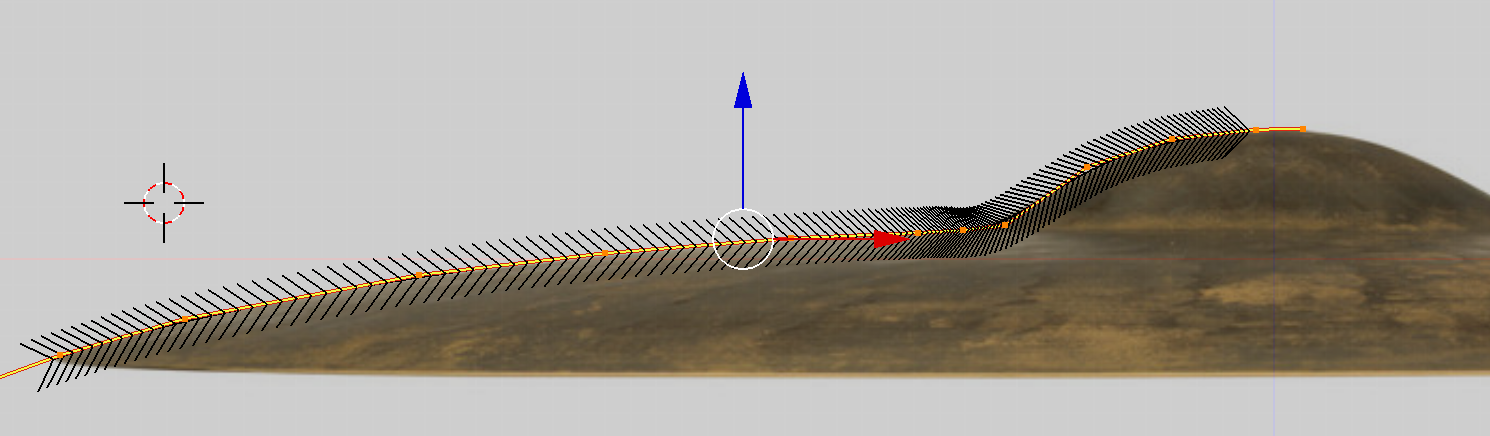
\includegraphics[width=\textwidth]{nurbs}
    \caption{\label{fig:nurbs}}
    %\vspace{-0.3cm}
\end{figure}

Una volta ottenuto il profilo perfetto, occorre convertire la curva in un oggetto mesh (alt + C) per poter effettuare lo \textit{spinning}. 

\begin{wrapfigure}{l}{0.3\textwidth} %this figure will be at the rightù
    \centering
    \vspace{-0.7cm}
    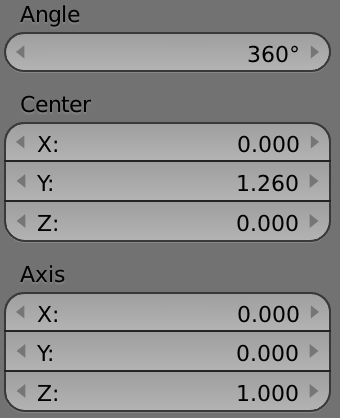
\includegraphics[height=5.5cm]{spin-values}
    \caption{\label{fig:spin-values}}
    \vspace{-3.7cm}
\end{wrapfigure}

\vspace{1cm}Come si può notare in figura \ref{fig:spin-values} è stata applicata una rotazione di 360\degree, è stato preso un centro di rotazione leggermente rialzato con un asse di rotazione unico $Z$.
La curva è stata traslata leggermente verso sinistra per poter lasciare un buco in alto. Questo buco serve per inserire il piatto su un asta che lo sorregge.\\

\newpage

Il risultato ottenuto è il seguente. Si può notare la differenza tra la versione flat e la versione smooth. Nell'immagine con la versione flat si può notare ancora la NURBS trasformata in mesh.\\

\begin{figure}[hbt]%
	\vspace{-1cm}
    \centering
    \subfloat[Piatto Flat]{{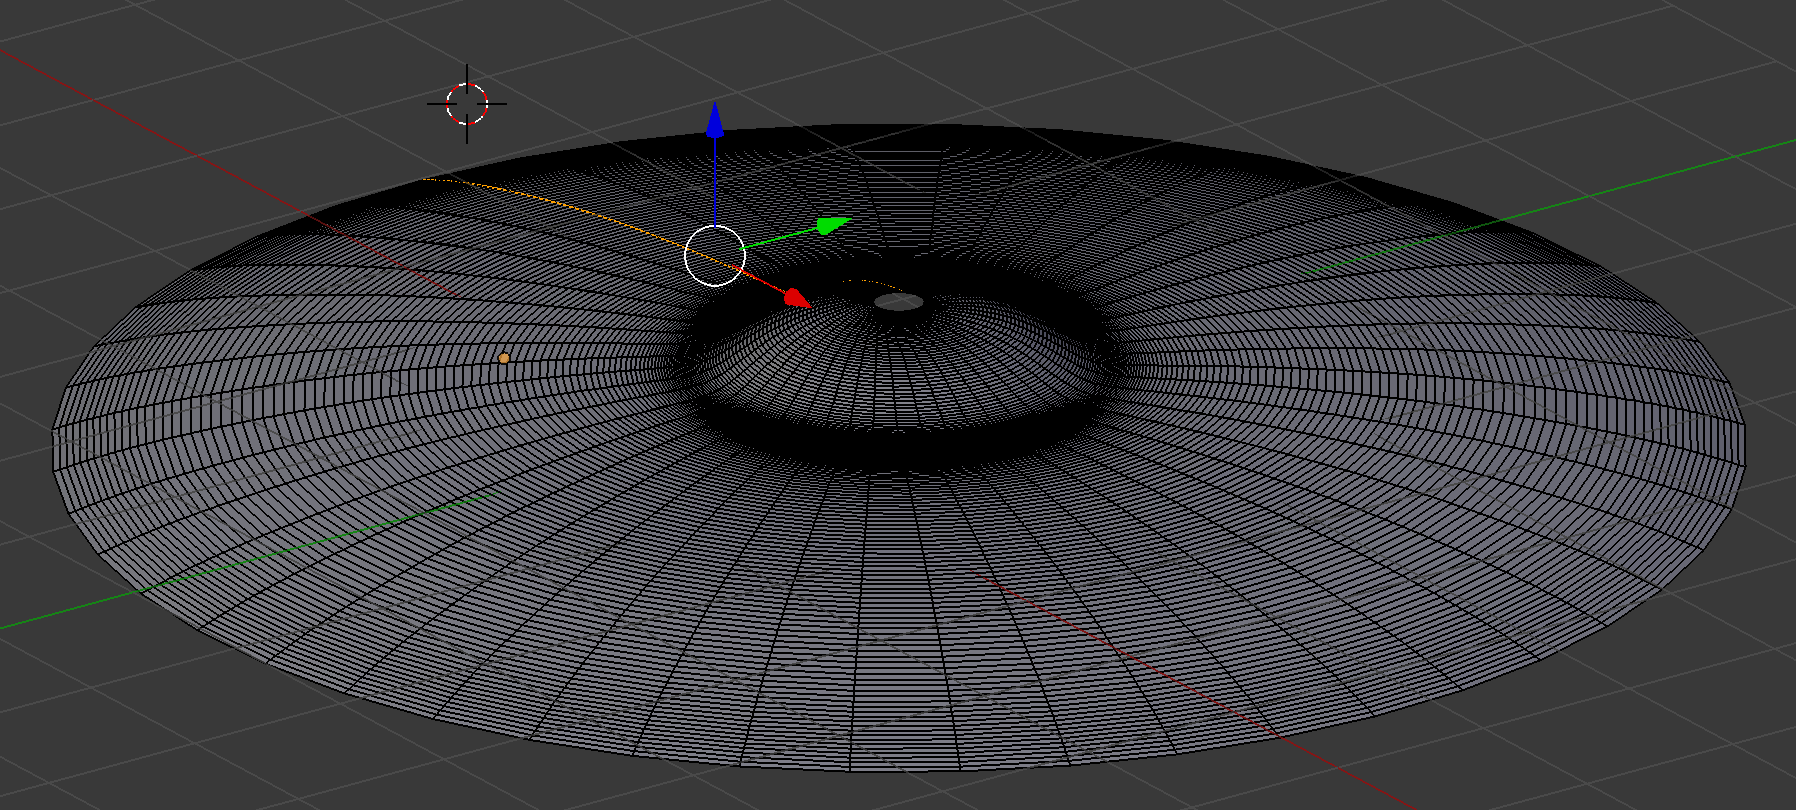
\includegraphics[height=4cm]{cymbal-flat} }}%
    \subfloat[Piatto Smooth]{{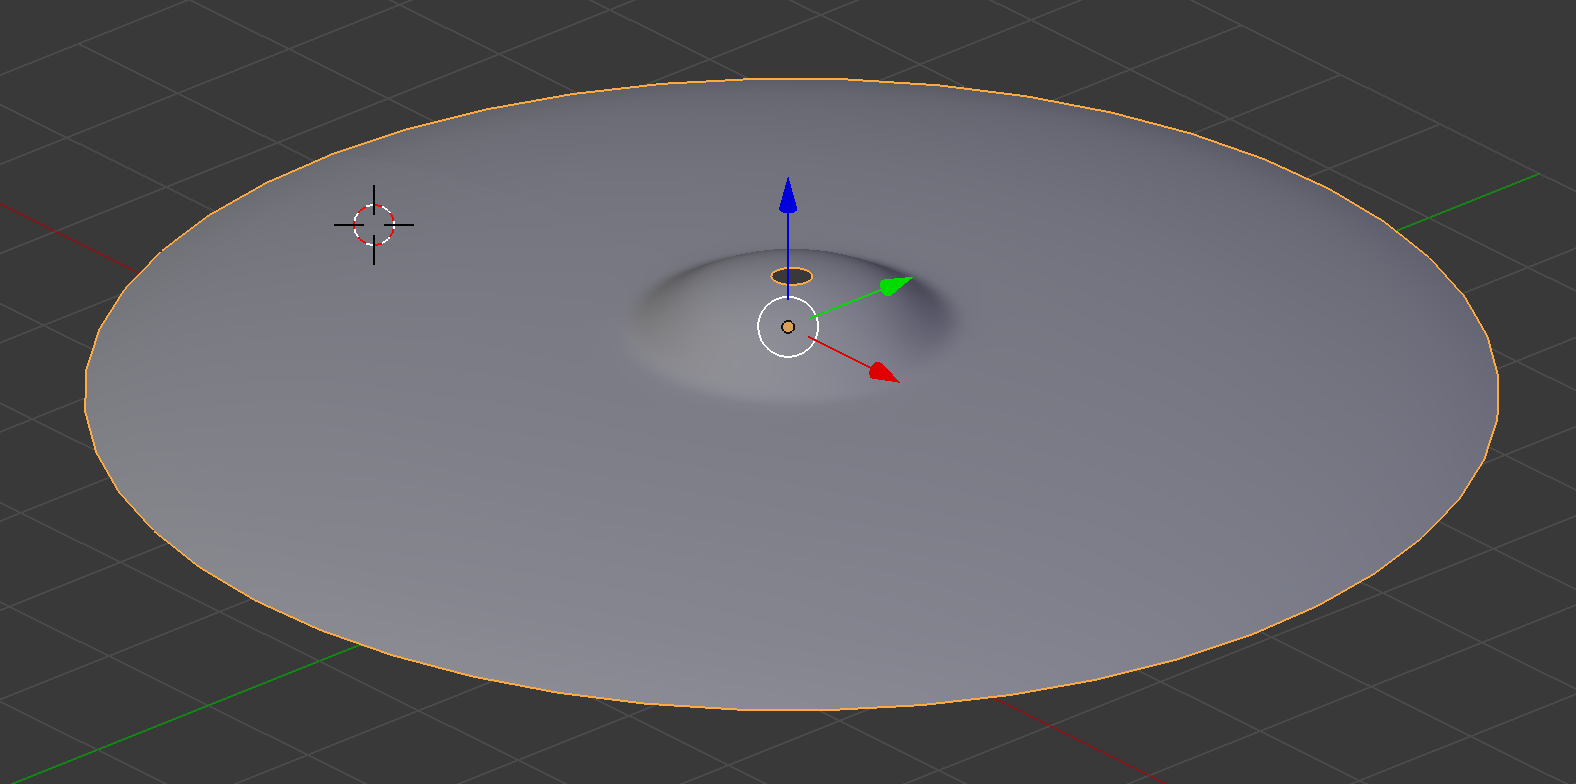
\includegraphics[height=4cm]{cymbal-smooth} }}%
	\vspace{-0.2cm}
\end{figure}



%===========================
\section{Parte 2 - MeshLab}
